\documentclass[12pt,a4paper]{report}

%###################################################################################
%###################### Document Defintions ########################################
%###################################################################################
%aubrey: no real need to change these
%how to handle spaces
\sloppy
\makeindex

\usepackage[latin1]{inputenc}
\usepackage{amsmath, marvosym} % Mathematik
%\usepackage{harvard} %for harvard style citation, keep this position before url package
\usepackage{times, url, geometry, amssymb, booktabs}
\usepackage[hidelinks]{hyperref} %Hyperlinks zw. Textstellen
\usepackage[pdftex]{graphicx} %pdf figures
\usepackage{subfig} %multi-figures
\usepackage{listings} %code listings
\usepackage{multirow} %for multi-row tables
\usepackage{color} %needed for listings
\usepackage{caption}

%\setlength{\parindent}{0pt} % no intendation for paragraphs

\DeclareCaptionFont{white}{ \color{white} }
\DeclareCaptionFont{black}{ \color{black} }
\DeclareCaptionFormat{listing}{
  \colorbox[cmyk]{0, 0, 0, 0}{
    \parbox{\textwidth}{\hspace{15pt}#1#2#3}
  }
}
\captionsetup[lstlisting]{ format=listing, labelfont=black, textfont=black, singlelinecheck=false, margin=0pt, font={bf,footnotesize} }

\usepackage{fancyvrb}
\DefineVerbatimEnvironment{code}{Verbatim}{fontsize=\small}
\DefineVerbatimEnvironment{example}{Verbatim}{fontsize=\small}

\definecolor{Grey}{rgb}{0.83,0.83,0.83}
\definecolor{White}{rgb}{1,1,1}
% predefined colors for source-code
\definecolor{darkred}{rgb}{.6,0,0}
\definecolor{darkmagenta}{rgb}{.6,0,.6}
\definecolor{darkgreen}{rgb}{0,.6,0}
\definecolor{turqoise}{cmyk}{0.9,0,0.2,0.3}

\newcommand{\nessi}{\texorpdfstring{\textit{NeSSi\textsuperscript{2}}}{NeSSi 2}}
\newcommand{\nessiUI}{\nessi{} User Interface}

\newcommand{\lineFive}[6]{\cellcolor{#1}#2&\cellcolor{#1}#3&\cellcolor{#1}#4&\cellcolor{#1}#5&\cellcolor{#1}#6\\}

\newcommand{\whiteLineFive}[5]{\lineFive{White}{#1}{#2}{#3}{#4}{#5}}
\newcommand{\blueLineFive}[5]{\lineFive{Grey}{#1}{#2}{#3}{#4}{#5}}


\interfootnotelinepenalty=10000

% setup of code-evironments
\lstloadlanguages{Java,XML}

% Defines an XML-Code-Environment
% usage: 
% \begin{xml} 
%   your code 
% \end{xml}
\lstnewenvironment{xml}{
\vspace{0.1em}\fontfamily{pcr}\selectfont
	\lstset{
	  language=XML,
		basicstyle=\scriptsize,
	  commentstyle=\itshape\color{darkgreen},
	  keywordstyle=\bfseries\color{darkred},
	  stringstyle=\tt\color{blue},
	  showspaces=false,
	  showtabs=false,
	  columns=fixed,
	  numbers=none,
	  frame=single,
	  numberstyle=\tiny,
	  breaklines=true,
	  showstringspaces=false,
	  tabsize=3,
	  moredelim=**[s][\bfseries\color{darkred}]{<}{>},
	}
}
{\normalfont\selectfont}

%depth of section
\setcounter{secnumdepth}{4}
%depth of TOC
\setcounter{tocdepth}{3} 
%directory for graphics
\graphicspath{{gfx/}}

%setting for listing
\lstset{
	extendedchars=true,
	basicstyle=\scriptsize\ttfamily,
	%basicstyle=\tiny\ttfamily,
	tabsize=2,
	keywordstyle=\textbf,
	commentstyle=\color{grau},
	stringstyle=\textit,
	numbers=left,
	numberstyle=\tiny,
	% für schönen Zeilenumbruch
	breakautoindent  = true,
	breakindent      = 2em,
	breaklines       = true,
	postbreak        = ,
	%prebreak         = \raisebox{-.8ex}[0ex][0ex]{\ensuremath{\lrcorner}},
	prebreak         = \raisebox{-.8ex}[0ex][0ex]{\Righttorque},
}

%Table of Content TOC settings
\setcounter{tocdepth}{3}
%This is needed for entering URLs for harvard citation style
%\renewcommand{\harvardurl}{URL: \url}


%###################################################################################
%########################### Thesis content ########################################
%###################################################################################
\begin{document}
%__________________________Start_of_Thesis______________________________________________
%Roman numeral numbering for initial section of thesis
\pagenumbering{roman}
%title page specification, deployed as seperate file the input folder
%############################################################################
%########################### Change This ####################################
%############################################################################
%put your title here
\newcommand{\trtitle}{Outlier Intrusion Detection System}
%replace with "Bachelor Thesis", "Master Thesis" or "Diplomarbeit"
\newcommand{\trtype}{Intelligente Sicherheit in Netzwerk (InSiN) Project Report}
%your name
\newcommand{\trauthor}{Alwin Alwin, Dmytro Gerasymchuk, \\ Evgeny Bardin, Nesrine Doghri}
% your matrikelnummer
\newcommand{\trmatrikelnummer}{309736}
%supevisor
\newcommand{\trbetreuerA}{Dr.-Ing. Karsten Bsufka}
%estimator 1
\newcommand{\trguta}{Prof.\ Dr.\ Dr.\ h.\ c.\ Sahin Albayrak}
%estimator two
\newcommand{\trgutb}{Prof.\ Dr.\ habil.\ Odej Kao}
\newcommand{\trdate}{\today}

%############################################################################
%########################### DO NOT touch this, unless you need to ##########
%############################################################################
\thispagestyle{empty}
%head line logo + tub + logo
\begin{tabular}{lcc}
\includegraphics[width=0.15\textwidth]{template/TUBerlin_Logo_rot_hell}& \hspace{1.1cm} Technische Universit{\"a}t Berlin& \hspace{1.2cm} 
\includegraphics[width=0.15\textwidth]{template/aot_logo}\\
\end{tabular}
%draw a line
\rule{\textwidth}{0.4pt}
%aub: remove this on final submission

%vertical space
\vspace{2.5cm}
\begin{center}
%replace this
  \textbf{\LARGE \trtitle}
\end{center}
\vspace{2cm}

\begin{center}
  \textbf{\trtype} \\
  Fachgebiet Agententechnologien in betrieblichen Anwendungen und der Telekommunikation (AOT)\\
  Prof.\ Dr.\ Dr.\ h.\ c.\ Sahin Albayrak \\
  Fakult{\"a}t IV Elektrotechnik und Informatik \\
  Technische Universit{\"a}t Berlin \\[0.5cm]
  submitted by \\
  \textbf{\trauthor}
\end{center}

\vspace{0.005cm}

\begin{center}
	\textbf{Group-03}
\end{center}

\vspace{1cm}

\begin{center}
\begin{tabular}{ll}
Supervisor:& \trbetreuerA\\
\end{tabular}
\end{center}

\vfill

\begin{tabular}{l}
\trauthor \\
\end{tabular}

\rule{\textwidth}{0.4pt}

\clearpage

%abstract plus acknowledgement and statement
%%#############################################################
%###################### Statement ############################
%#############################################################
\chapter*{Plagiatserkl{\"a}rung}
%this one needs to be signed for submission
    Hiermit versichern wir, dass wir die vorliegende Arbeit \"{u}ber \textbf{Recent Research Trends of Artificial Immune Systems for IT-Security} selbst\"{a}ndig verfasst und nur die angegebenen Quellen und Hilfsmittel verwendet habe. Stellen der Arbeit, die anderen Werken -- auch elektronischen Medien -- dem Wortlaut oder Sinn nach entnommen wurden, habe ich unter Angabe der Quelle kenntlich gemacht.

\vspace{4cm}

\noindent Berlin, 29 Juli 2015 \hfill Signature

%#############################################################
%###################### German Abstract ######################
%#############################################################
%\newpage
%\chapter*{Zusammenfassung}
    
%    \textbf{Schlagw\"orter:}
%#############################################################
%###################### Abstract  ############################
%#############################################################
\newpage
\chapter*{Abstract}

    The field of intrusion detection has grown rapidly due to the growing concern of IT security.\ Perhaps the most important characteristic of the biological immune system is that it is particularly robust in defending the host against invading agents and at the same time especially impeccable in recognising and distinguishing between self and non self cells.\ By taking inspiration from the biological immune system, the artificial immune system (AIS) shows a promise to deliver solutions to the issue of IT security, especially in detecting intrusion.\ This paper introduces and describes three recent papers published in the field of AIS for IT security from the International Conference on Artificial Immune System (ICARIS) 2012.\ A subjective evaluation of each works is then presented in conclusion of this paper.
    
    \noindent\textbf{Keywords:} Artificial Immune System, AIS, IT-Security  
    
    
%DELETEME: An abstract is a teaser for your work. You try to convince a reader that it is worth reading your work. Normally, it makes to structure you abstract in this way: 
%\begin{itemize}
%\item one paragraph on the motivation to your topic
%\item one paragraph on what approach you have chosen
%\item and one paragraph on your results which may be presented in comparison to other approaches that try to solve the same or a similar problem.
%\end{itemize}
%Abstract should not exceed one page (aubrey's opinion)

%DELETEME: translate to German to Englisch or vice-versa.

%#############################################################
%###################### Acknowledgements #####################
%#############################################################
%\newpage
%\chapter*{Acknowledgements}

%DELETEME: Thank you for the music, the songs I am singing
    %The author expresses his gratitude towards Dipl.-Ing.\ Jo\"{e}l\ Chinnow and Dr.-Ing.\ Karsten\ Bsufka as his supervisors for their guidance and supports during the thesis. The author also wishes to thank his colleagues, Leily\ Behnam\ Sani\ and The\ Hieu\ Tran\ for their assistance and valuable ideas to the undertaking of the work summarized here.
    
    
    

%TOC
\tableofcontents
%add list of figures to TOC
\cleardoublepage
\addcontentsline{toc}{chapter}{List of Figures}
\newpage
\listoffigures
%add list of tables to TOC
%\cleardoublepage
%\addcontentsline{toc}{chapter}{List of Tables}
%\newpage
%\listoftables

%__________________________Main_Content______________________________________________
\newpage
%from now on, numbering should be arabic
\pagenumbering{arabic}
\chapter{Introduction}
\label{introduction}

	Due to the rapidly expanding IT-infrastructure and ,thus, its complexity, IT-security has become a concern that poses increasingly difficult challenges for IT-security experts in protecting the system from malicious attacks.\ One major contributing factor is the growing complexity of cyber-attacks which, assisted by automation development, lowers the required knowledge to perform such attacks even further \cite{McHugh:IntrusionAndIntrusionDetection}.\ In order to deal with this phenomena, various cyber-defence mechanisms and tools have been developed over the years, one of which is \textit{intrusion detection system}.
	
	An intrusion detection system (IDS), proposed by Denning in 1987 \cite{Denning:IntrusionDetectionModel}, is a system that aims to detect intrusion (security-breach) into a system and fires an alert in order for security-personals to decide on necessary course of actions.\ While there has been significant amount of research in the field of IDS, it remains a young research-field and is still plagued by several weaknesses, such as high false positive rates.
	
	This project aims to tackle the task of developing an IDS system in order to be familiarised with the challenges of IDS-development as well as to be able to recognise both the strength along with the weaknesses of different IDS-strategies/-mechanisms.\ The goal of this project is to develop an IDS system that has the capability to identify malicious (anomaly) behaviour in the IT-infrastructure and provides an alert accordingly.
	
	This project report is structured as follows.\ Chapter~\ref{background} explains some necessary background that is required to understand the work of this project, Chapter~\ref{objectives} sets the objectives which are relevant in order to achieve the goal of this project; Chapter~\ref{approach} describes the approach of the authors to reach the objectives; The actual implementation details are explained in Chapter~\ref{implementation} whereas the performance of the implementation is described in Chapter~\ref{results}.\ Finally, Chapter~\ref{conclusion} sums up this project and provides some insight to future works related to this project.

\chapter{Background}
\label{background}

	In computer security, intrusion detection is the fact of detecting malicious actions that attempt to compromise the confidentiality, integrity or availability of a resource. Intrusion detection can be performed manually or automatically.\ In the process of manual intrusion detection, a human examines log files to find any suspicious sign that can indicate an intrusion.\ A system that performs the automated intrusion detection is called intrusion detection system (IDS).

	In this chapter, we will take a deeper look on the Intrusion detection systems. We will explain the possible categories of those systems in the first section, present the available datasets to evaluate them in the second section and give a brief overview of the algorithms used in our project in the remaining sections.

	\section{Intrusion detection systems (IDS)}

		An intrusion detection system is a mechanism intended to analyse the security status of an information system in order to detect anomalies or suspicious activities.

		\subsection{Typical Components }

			As described in \cite{BSI}, the software components of an Intrusion Detection System can be be grouped, according to their functions, into four types:

			\begin{description}
				\item[- Sensors:] They are responsible for collecting  events from host or network-based data sources and transmitting them for further analysis and storage.

				\item [- Evaluation stations:] They analyze the events and identify the attacks. The evaluated informations will be also transmitted as events, which allows repeated analysis. 
				\item [- Management stations:] They regulate the communication between the individual components of an IDS, determine the necessary parameters, monitor the individual event streams and send warning messages.
				\item [- Database Components:] They are used to efficiently manage and store the collected data of all components.

			\end{description}

		\subsection{IDS Taxonomy}

			As presented in figure \ref{Taxonomy of intrusion detection systems}, IDS systems could be classified into four categories.

			\begin{figure}[h!]
				\centering
				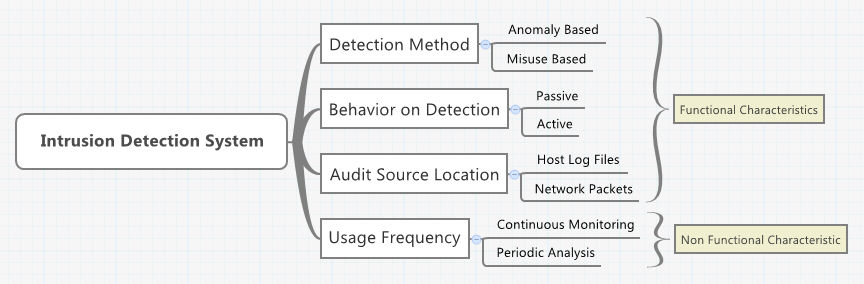
\includegraphics[scale=0.45]{figures/Taxonomy.png}
				\caption{Taxonomy of intrusion detection systems}
				\label{Taxonomy of intrusion detection systems} 	
			\end{figure}
				
			The network security tool uses either of two main approaches to detect the anomalies.\ The first one, anomaly based, explores issues in intrusion detection associated with deviations from normal behaviour of the monitored system.\ The second approach uses informations about attacks to discriminate between anomaly or attack patterns.\ After detecting an attack, an active IDS tool can automatically block suspected attacks in progress (known as an intrusion response system), whereas a passive IDS can only alert an operator to potential vulnerabilities and attacks and log network packets.

	
			Intrusion detection systems can be classified according to the source of data.\ An IDS tool can either use informations derived from a single host: host based IDS (HIDS) and or exploit informations obtained from a whole segment of a local network (network based IDS, i.e. NIDS).


			An IDS tool can be characterized by its usage frequency, we distinguish between a dynamic IDS that runs on a continuous feed of information and performs real-time analysis and a static IDS that periodically takes a snapshot of the environment and analyzes it.


		\subsection{Detection Methodologies}

			In this section we discuss the primary classes of detection methodologies: Misuse-based based and Anomaly based.

			\subsubsection{Misuse-based intrusion detection}

				The Misuse-based intrusion detection system possesses patterns describing known attacks called signatures.\ It is the simplest detection method as it identifies possible attacks by just comparing those signatures against observed events. 


				While these systems are very effective at uncovering known attacks with a few number of false alarms, they are not able to detect novel attacks for which the signatures are not yet available, therefore the signatures must be constantly updated.\ Two approaches are commonly used to implement this technique: 

				\begin{description}

					\item[\textbf{- Pattern matching approach:}] In this approach attack patterns are modelled, matched and identified based on the packet header and/or packet content.
					\item[\textbf{- Rule-based approach:}] This approach makes use of expert systems that contain a set of rules describing the attacks, which are matched against audit or network traffic data.\ Any deviation in the rule matching process is reported as an intrusion.

				\end{description}
	
			\subsubsection{Anomaly detection} 

				Anomaly detection constructs normal activity profiles for the system during a training phase and then considers any current behavior that does not match the stored profile as a suspicious action.\ These systems are able to detect novel attacks, but they generally have a substantial false alarm rate and the training of a very dynamic system requires a constant update of the normal behaviour profile database.\ According to \cite{AnomalyBasedNID} anomaly detection techniques can be grouped into three main approaches:

				\begin{description}
					\item[\textbf{- Statistical-based techniques:}] A user or a system profile reflecting its behavior is constructed by measuring a number of variables sampled over time.
					\item[\textbf{- Knowledge based techniques:}] They require the availability of prior knowledge. The expert system approach is one of the most widely used Knowledge based schemes.
					\item[\textbf{- Machine Learning techniques :}] They are widely used in the anomaly based intrusion detection since they enable to automatically construct a model that reflects the subject's normal behavior. They fall into two categories: supervised and unsupervised learning.

						\begin{itemize}
							\item { \textbf{Supervised learning:}} It proceeds in two steps, first in the training phase a classification model is learned based on datasets labeled with predefined classes . Then, in the testing phase, ths classification model is used to predict the classes of new instances. SVM, neural networks, Bayesian network are some of the widely used supervised learning techniques. Section \ref{svmSection} will be dedicated to better explain the support vector machines.
							\item { \textbf{Unsupervised learning:}} They try to detect intrusions without using any prior knowledge of attacks or normal instances.\ Clustering and outlier detection based techniques are among the most popular approaches suggested.\ Among the clustering strategies we find the K-means approach which will be further discussed in section \ref{kmeans}.

						\end{itemize}
				\end{description}

			\subsection{Data source locations} 
				
				Intrusion detection systems can be categorised into two groups based on the location of the data source: network-based IDS or host-based IDS.

				\subsubsection*{Host based IDS}

					In this case, informations on the activities of the users of a given machine are gathered based only on the Host audit sources, for example: system commands like: \textit{vmstat}, \textit{pstat}; Syslog audit service.
				 
				\subsubsection*{Network based IDS}

					A network-based IDS collects informations from the network traffic streams  as data is transmitted between particular network segments, suspicious activities are identified inspecting the contents and header informations of all the packets transferred across those segments.\ In the following we'll give a brief overview of the TCP/IP protocol suite and then we will cover the major components of network-based IDSs.

					\begin{enumerate}
						\item{\textbf{Transmission Control Protocol}}
						
							To provide network communication the internet protocol stack is composed of 4 layers: the data link, network, transport, and application layers.\ When a user wants to transfer data across networks, the data is passed through all the layers starting from the application layer, with each layer encapsulating  more header informations.\ The data link layer sends the packet through the physical network; when received by a host the data gets decapsulated as it is passed up  through the layers.

							The TCP protocol is a connection oriented transport protocol, that is, the sender and the receiver processes must handshake with each other by exchanging control messages initialzing many state variables contained in the TCP header before establishing the connection.

							Figure \ref{tcp} depicts the TCP headers as defined in RFC 793.
								\begin{figure}[h!]
									\centering
									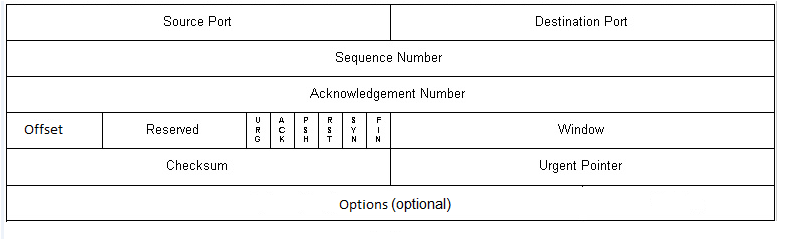
\includegraphics[scale=0.66]{figures/TCP.png} 
									\caption{TCP Header}\label{tcp} 	
								\end{figure}

							The source and destination ports contain respectively the source and the destination port number of the packet.\ For each TCP connection, numbers are negotiated between the communication partners.\ The sequence number field contains the number of first byte in segment's data.\ The acknowledgment number is the sequence number of the next byte expected from the other side, thus the sender can determine whether the data arrived at the receiver.
							
					\begin{table}[h!]
						\centering
  						\resizebox{\textwidth}{!}{ 						
							\begin{tabular}{|c|c|p{6cm}|}
								\hline 
								\textbf{Flag} & \textbf{Meaning} & \textbf{Function} \\ 
								\hline 
								$URG$ & Urgent & Set if data is urgent \\ 
								\hline 
								$ACK$ & Acknowledgment & Acknowledges the received data \\ 
								\hline 
								$PSH$ & Push & Informs the receiving host that the data should be immediately pushed up to the receiving application  \\ 
								\hline 
								$RST$ & Reset & Reset the connection in response to an invalid segment \\ 
								\hline 
								$SYN$ & Synchronise & Initiates a connection \newline
								$SYN$ = 1, $ACK$ = 0 for connection request;\newline 
								$SYN$ = 1, $ACK$ = 1 for acknowledgment of receipt\\ 
								\hline 
								$FIN$ & Finish & Closes a connection\newline
								$FIN$ = 1, ACK = 0 Disconnection request;\newline 
								$FIN$ = 1, ACK = 1 Confirmation \\ 
								\hline 
							\end{tabular} 
						}
								\caption{TCP Flags} \label{flags}
						\end{table}				

						\item {\textbf{Architecture overview:}}\\
						
							The network IDS usually has two logical components: the sensors and the management station \cite{guide}.\\
							
							\begin{description}
								\item[- The sensors:] They are on the network segments, they are dedicated to monitor them for suspicious traffic.\ Their network interface is set in the promiscuous mode, which means they receive all network traffic.\ If they detect a suspicious packet, they send it to the management station.
								\item[- The management station:] It receives alarms from the sensor(s), stores them in the Simple Network Management Protocol (SNMP) Management Information Base (MIB).\ It can perform some additional analysis and display them to the network administrator.
							\end{description}

							The placement of the sensors and the management station is shown in Figure~\ref{archi}.

							\begin{figure}[h!]
								\centering
								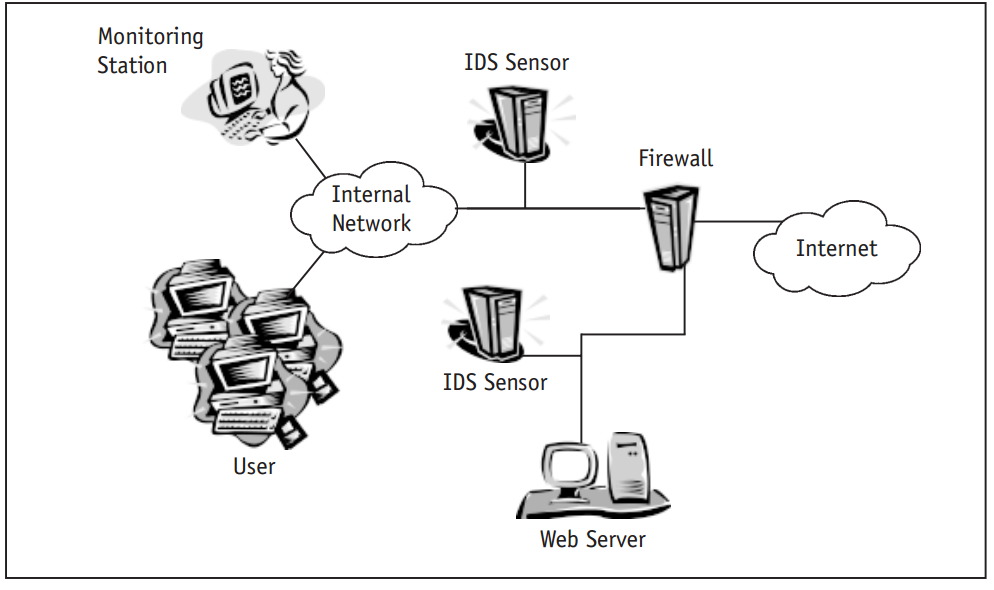
\includegraphics[scale=0.5]{figures/NIDS.PNG} 
								\caption{Network based IDS architecture \cite{guide}}
								\label{archi} 
							\end{figure}
					\end{enumerate}
		
		\section{Available Datasets} 

			Datasets are utilized to evaluate the performance of Intrusion Detection Systems.\ There are two publicly available datasets: The DARPA datasets developed by the MIT Lincoln Labs and the KDD Cup dataset derived from them, they both consist of US air force local network data with a variety of simulated attacks.

				\subsection{DARPA Datasets}
				
					The DARPA datasets were built by MIT Lincoln Laboratory in 1998 and 1999 in the context of a project supported by DARPA aiming to provide a source of data that enables to quantitatively evaluate Intrusion detection systems.\ They performed a simulation of an Air Force base connected to the Internet.

					The 1999 Off-line Simulation Network architecture is depicted in figure \ref{DARPA archi}.\ As shown in the figure, the simulation network has two segments where the left side represents the networks inside of the simulated Eyrie Air Force Base, it includes victim machines with different operating systems and a gateway to other inside workstations and the right side represents the Internet outside the base. 

					\begin{figure}[h!]
						\centering
						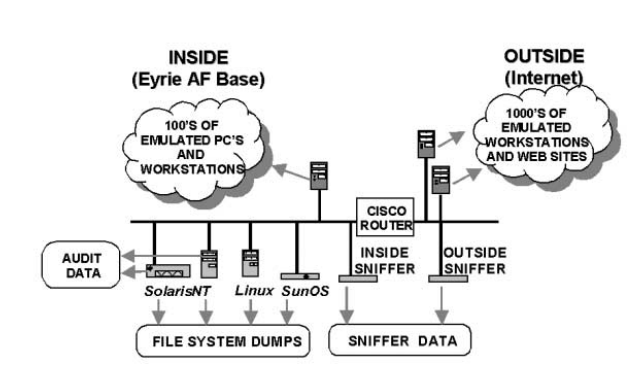
\includegraphics[scale=0.7]{figures/Network.PNG}
						\caption{DARPA'$99$ simulation network architecture}
						\cite{DARPAEvaluation}
						\label{DARPA archi}	
					\end{figure}
						
					The test bed network generated three weeks of training data with background traffic and labeled attack, the first and third weeks of the training data can be used in the training of anomaly detection systems as they do not contain any attacks, and two weeks of test data with background traffic and unlabelled attacks.\ The attacks used in the simulations can be divided into four categories \cite{ComparativeStudy}, namely:

					\begin{itemize}
						\item {Probing:} Attacks that attempts to gather information about network of computers or find known vulnerabilities.
						\item {Denial of Service (DoS):} Attacks that deny legitimate requests from legal users on the system by making full usages of computing or memory resources.
						\item {User to Root (U2R):} Attacks that exploit the vulnerability of the system to obtain root access to it from a normal user privilege.
						\item {Remote to Local (R2L):} Attacks that exploits the vulnerability of the system to gain a local user account launching remote exploits.
					\end{itemize}
					
					The procedures used in building the dataset and in performing the evaluation were criticized by MacHugh \cite{DARPACritique}.

				\subsection{KDD Dataset}

					The KDD dataset is a labeled version of 1998 MIT DARPA dataset where data packets forming a complete session were gathered in a single feature vector.\ KDD records have 41 features, defined for each connection samples which can further be classified into three groups namely: basic features, traffic features, content features \cite{Mahbod:KDD}.\ The goal of this dataset was to demonstrate the applicability of different knowledge discovery and machine learning techniques on intrusion detection systems.

		\section{Principal Component Analysis}

			Principal Components Analysis is a technique introduced by Pearson and Hotelling that aims to reduce the dimensionality of multivariate data while preserving as much as possible of the present variation.

			It is an unsupervised learning approach that only relies on the input data.\ PCA transforms a large number of variables to a new reduced set of variables, the principal components, that are uncorrelated and linear functions of the original variables, such that, the greatest variance by any projection of the data comes to lie on the first coordinate, the second greatest variance on the second coordinate, and so on.
			
			In practice, this is achieved by computing the covariance matrix for the full data set.\ Next, the eigenvectors and eigenvalues of the covariance matrix are computed, and sorted according to decreasing eigenvalue.\ This approach can be inappropriate for some applications as features with low variance might actually have high predictive relevance \cite{pca}.

		\section{Support Vector Machines}
		\label{svmSection}

			SVMs have been introduced in 1992 at the COLT conference by Boser, Guyon, Vapnik as a supervised learning approach used to solve classification and regression problems.

			The simplest kind of support vector machines called Linear SVM aims to find a hyperplane that optimally separates the training vectors into two classes by achieving the maximum separation, such that it will be equidistant to both datasets.\ Support vectors are defined to be a subset of the training data having the minimum distance to the hyperplane.\ An example of a simple linear SVM is illustrated in Figure~\ref{svm}.
				
				\begin{figure}[h!]
					\centering
					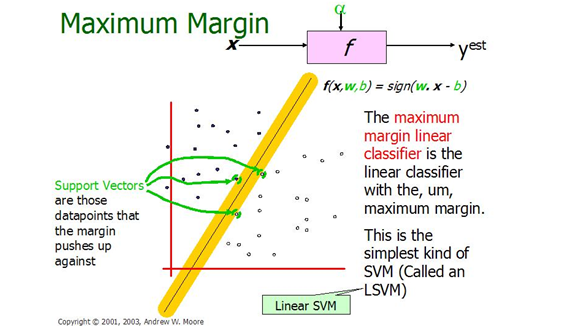
\includegraphics[scale=0.7]{figures/LSVM.PNG} 
					\caption{Linear Support Vector Machines \cite{SvmSlides}} \label{svm} 
				\end{figure}

			The goals of SVM are separating the data with a hyper plane and extend this to non-linear boundaries when the data is far from linear and the datasets are inseparable by using the kernel methods that allow SVMs to form nonlinear boundaries, by non-linearly mapping the input data to a high-dimensional space.\ The new mapping is then linearly separable \cite{Nello:Svm} \cite{Tom:MachineLearning}.

			The kernel functions enable operations to be performed in the input space rather than the potentially high dimensional feature space.\ Various kernel functions can be used \cite{Nello:Svm}, such as: \textit{Polynomial}, \textit{Gaussian Radial Basis Function}, as well as \textit{Exponential Radial Basis Function}.

			\subsection{One Class SVM}
		
			One Class SVM is an extension of the SVM methodology that handles training using only positive information, it identifies "outliers" amongst the positive examples and use them as negative examples \cite{Larry:OCSVM}. The OC-SVM algorithm maps input data into a high dimensional feature space using a kernel function and iteratively finds the maximal margin hyperplane which best separates the training data from the origin. It may be viewed as a regular two-class SVM where all the training data lies in the first class, and the origin is taken as the only member of the second class. Thus, the hyperplane (or linear decision boundary) corresponds to the classification rule. The decision function is given by:  \cite{Katherine:OCSVM}:

			\begin{equation}
				f(x) = <w,x> +b
			\end{equation}
			
			where \textit{w} is a vector perpendicular to the hyperplane and \textit{b} is a bias term. The OC-SVM solves an optimisation problem to find the decision function $f$ with maximal geometric margin.\ This function can be used to label a test example x as an anomaly if $[f(x)<0]$ and as normal otherwise. Solving the OC-SVM optimisation problem is equivalent to solving the dual quadratic programming problem:

			\begin{equation}
				\min_{\alpha} \frac{1}{2}\sum_{i,j}\alpha_{i}\alpha_{j}K(x_{i},x_{j})
			\end{equation}

			subject to the constraints

			\begin{equation}
				0 \leq \alpha_{i} \leq \frac{1}{v_{l}}
			\end{equation}
			
			and 
		
			\begin{equation}
				\sum_{i}\alpha_{i}=1
			\end{equation}

			where $\alpha_{i}$ is a Lagrange multiplier (or "weight" on example \textit{i} such that vectors associated with non-zero weights are called "support vectors" and solely determine the optimal hyperplane), \textit{v} is a parameter that controls the trade-off between maximising the distance of the hyperplane from the origin and the number of data points contained by the hyperplane, \textit{l} is the number of points in the training dataset, and $K(x_{i},x_{j})$ is the kernel function.\ Given a feature map:

			\begin{equation}
				\phi: X \longrightarrow \Re^{N}
			\end{equation}

			where $\phi$ maps training vectors from input space \textit{X} to a high dimensional feature space, the kernel function can be defined as:

			\begin{equation}
				K(x,y) = <\phi(x),\phi(y)>
			\end{equation}

			After solving for the dual problem, a set of model weights $\alpha_{i}$ can be obtained and the decision function for any test vector x can be given by :

			\begin{equation}
				f(x) = sgn (\sum_{i}\alpha_{j}K(x_{i},x_{j}) - \rho)
			\end{equation}
			
			where $\rho$ is the distance to the origin.

		\section{KMeans} \label{kmeans}

			Kmeans is an unsupervised learning algorithm that aims to organise data from a given training set into few clusters.\ The Kmeans algorithm proceeds in two steps: First $K$ data items from the set of data points are randomly chosen as initial centroids, then, in the second step, each data point is assigned to the cluster which has the closest centroid and each cluster centroid is moved to the mean of the points assigned to it.\ This second step is repeated until all data points are assigned to one of the $K$ clusters.

			The Kmeans algorithm proceeds in two steps: First K data items from the set of data points are randomly chosen as initial centroids, then, in the second step, each data point is assigned to the cluster which has the closest centroid and each cluster centroid is moved to the mean of the points assigned to it. This second step is repeated until all data points are assigned to one of the K clusters. \\

			\textbf{- Silhouette Value:}
			
				A silhouette is a graphical display for partition techniques which shows  which objects lie  well within their cluster, and which not. The average silhouette width provides an evaluation  of clustering validity and might be used to select an 'appropriate' number of clusters \cite{silhouette}.\\
			 For each data point $i$, the silhouette $s(i)$ is given by the equation \ref{SilEq}:
				
				\begin{equation} 
					s(i)=\frac{b(i)-a(i)}{\max(a(i),b(i))} 
					\label{SilEq}
				\end{equation}
						
				where $a(i)$ is the average dissimilarity of $i$ with all other data within the same cluster and $b(i)$ is the lowest average dissimilarity of $i$ to any other cluster, of which $i$ is not a member.
\chapter{Objectives}
\label{objectives}

	Based on the project goal which is to developed an IDS system to detect anomaly, potentially malicious, behaviours in an IT-system, various objectives were defined, which includes:
	
	\begin{itemize}
		\item{Extract relevant information from given data-sets}
		\item{Training of the IDS system using machine learning methods on the extracted information}
		\item{Testing of the IDS system on DARPA'$99$ data-sets}
	\end{itemize}
	
	These objectives merely serve as a rough guideline during the IDS-development process.\ A detailed approach taken by the authors in order to achieve the project goal is described and explained in the next chapter.

\chapter{Approach}
\label{approach}

	Having determined the objectives, the first step of the development process is designing the IDS system's architecture.\ The design involved in this project report is based on the work of Manandhar \cite{Manandhar:TowardsPracticalAnomalyBasedIDS}, which is illustrated in Figure~\ref{fig:originalArchitectureDesign}.
	
	\begin{figure}[hb]
	  \centering
	  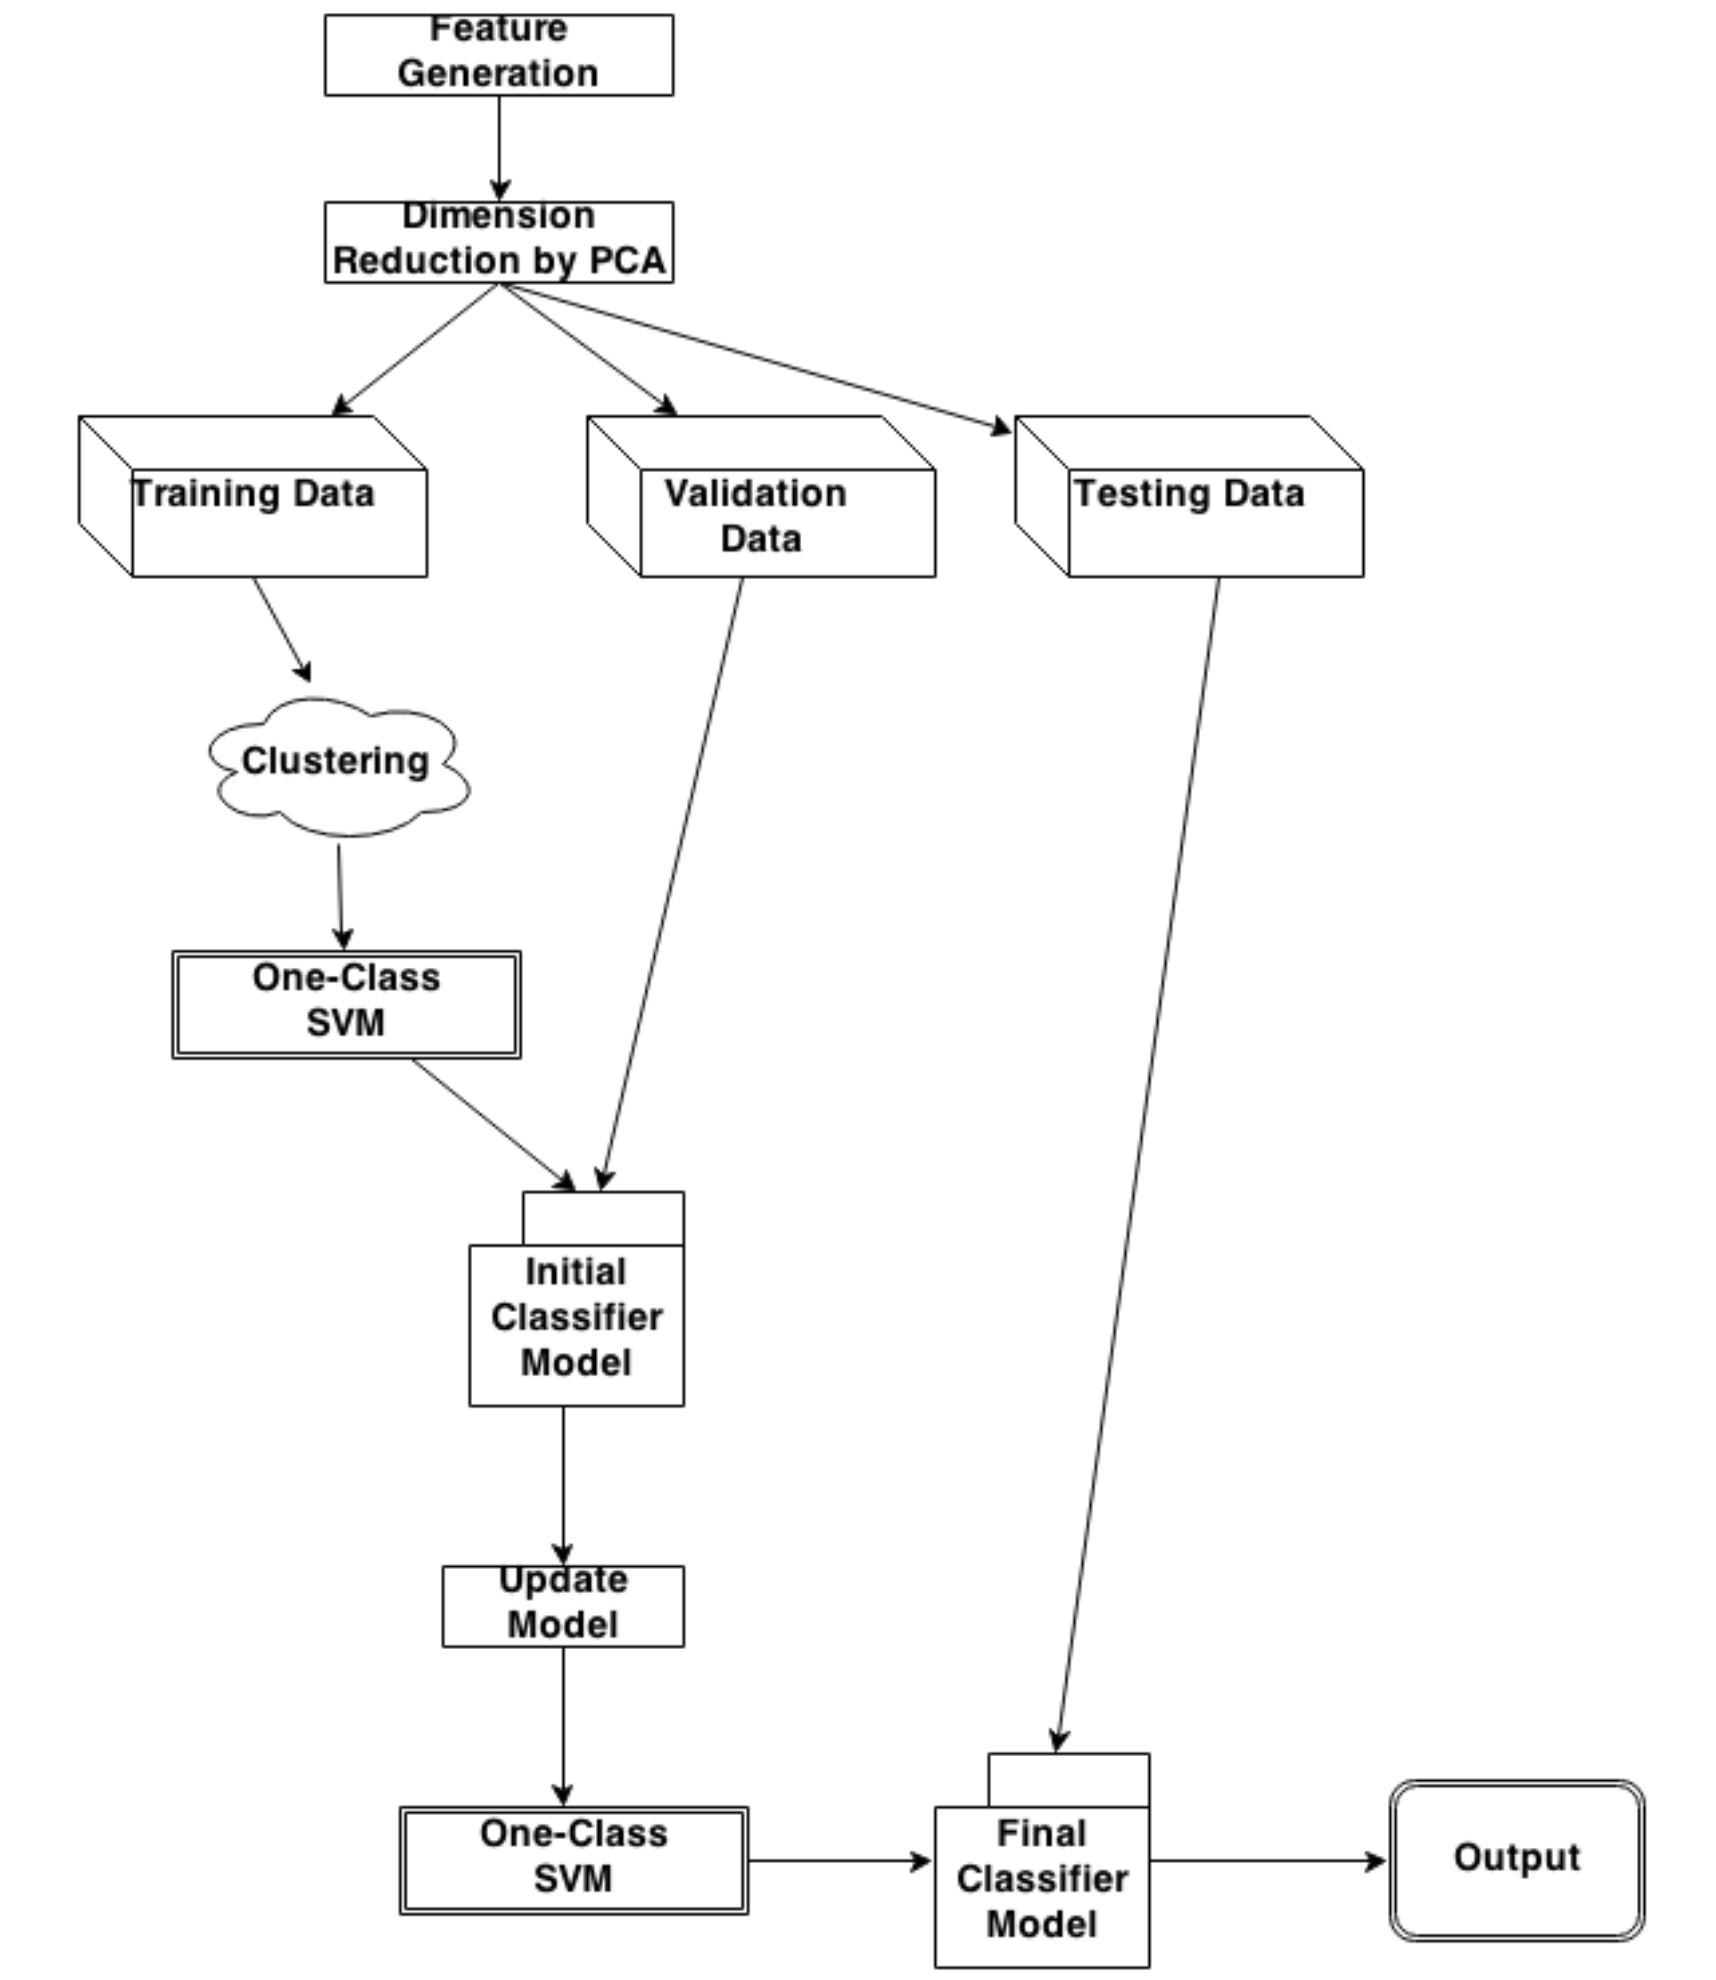
\includegraphics[scale=0.3268]{figures/OriginalArchitecture.png}
	  \caption{Architectural Design of IDS system \cite{Manandhar:TowardsPracticalAnomalyBasedIDS}}
	  \label{fig:originalArchitectureDesign}
	\end{figure}
	
	 The IDS system of this architectural design is set to work on real-time since it performs analysis only based on TCP/IP packet headers.\ The architecture consists of three main components, namely the data-sets preprocessing component, the training component and the testing (classification) component.\ This chapter describes the design of each component and its functionality.
	
	\section{Data-Set Preprocessing Component}

		The data-set preprocessing component is designed to perform extraction of relevant information from given data-sets.\ This component aims to increase the performance of the training component by providing only necessary information that is required to train the IDS system.\ Since the IDS system analyses only TCP/IP packet headers, all packet header information (e.g. payload size, flags, etc.) is extracted from the network packets which is contained in the data-sets. The complete workflow of data-set preprocessing component can be viewed on Figure~\ref{fig:activityDiagramPreprocessing}.

		\begin{figure}[hb]
	 	 \centering
		  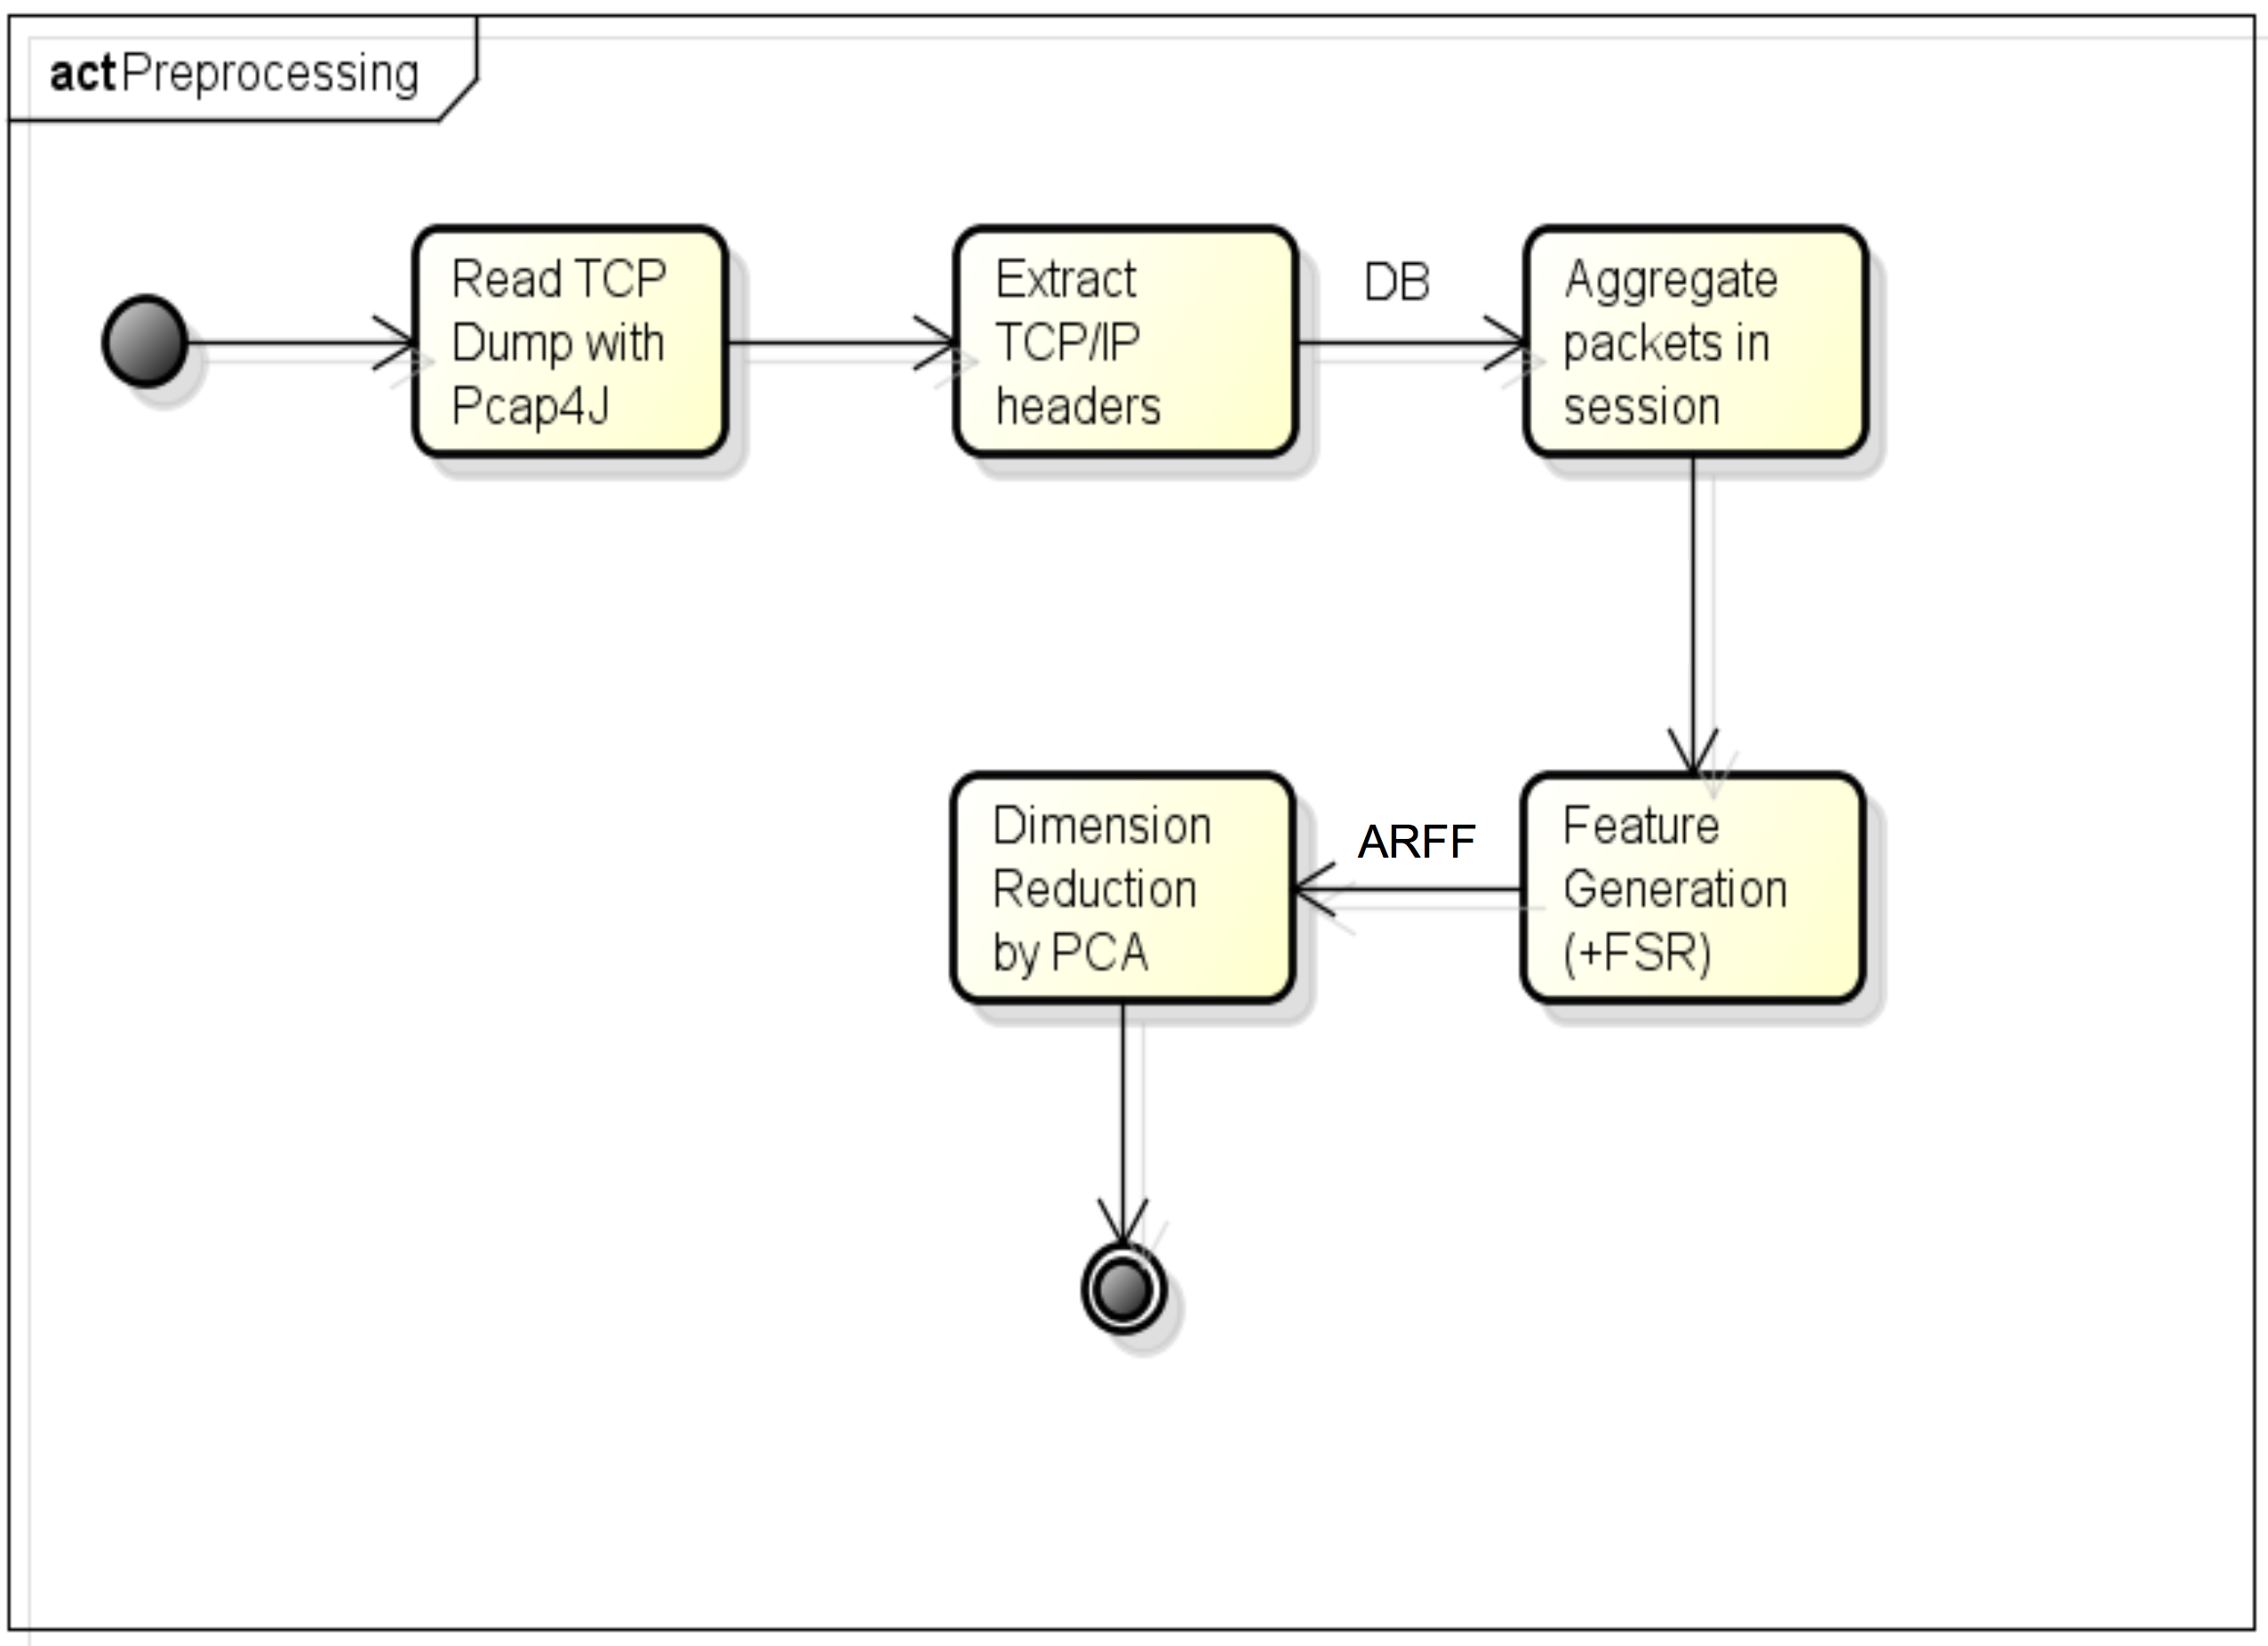
\includegraphics[scale=0.2668]{figures/ActivityDiagramPreprocessing.png}
		  \caption{Activity diagram describing the workflow of data-set preprocessing component}
		  \label{fig:activityDiagramPreprocessing}
		\end{figure}
		
		Preprocessing data-set starts by reading the data-set and converting each network packet into a $Java$ $Object$, which simplifies the header information extraction process.\ Due to the fact that a single abnormal network packet does not provide enough evidence regarding the nature of the network connection, the extracted header information from single packets has to be aggregated to represent one complete network-connection (\textit{TCP-session}).\ The aggregation process is done by building an average of each header information (e.g.\ average payload size, average count of $SYN$-flags, etc.) over four different characteristic of the network packet, namely \textit{source IP-address}, \textit{source port-number}, \textit{destination IP-address} and \textit{destination port-number}.\ This means that all network packets with the same characteristics mentioned above are aggregated into one TCP-session.
		
		Afterwards, the header information is utilised as feature vectors for the training component of the IDS system.\ However, in order to further improve the performance of the training component, the dimensions of these feature vectors are reduced with the help of principal component analysis (PCA).\ The resulting dimensional-reduced feature vectors are then passed onto the training component to be utilised as input for the IDS system's training process. 

	\section{Training Component}
		
		Clustering will be performed on the given dimensional-reduced feature vectors using $k$-$means$ method in order to determine the cluster centroids which serves as input for the one-class support vector machine. The resulting hyper-plane from one-class SVM is the IDS model, based on which the classification component functions.\ A corresponding activity diagram of this workflow is illustrated in Figure~\ref{fig:activityDiagramTraining}.
		
		\begin{figure}[hb]
	 	 \centering
		  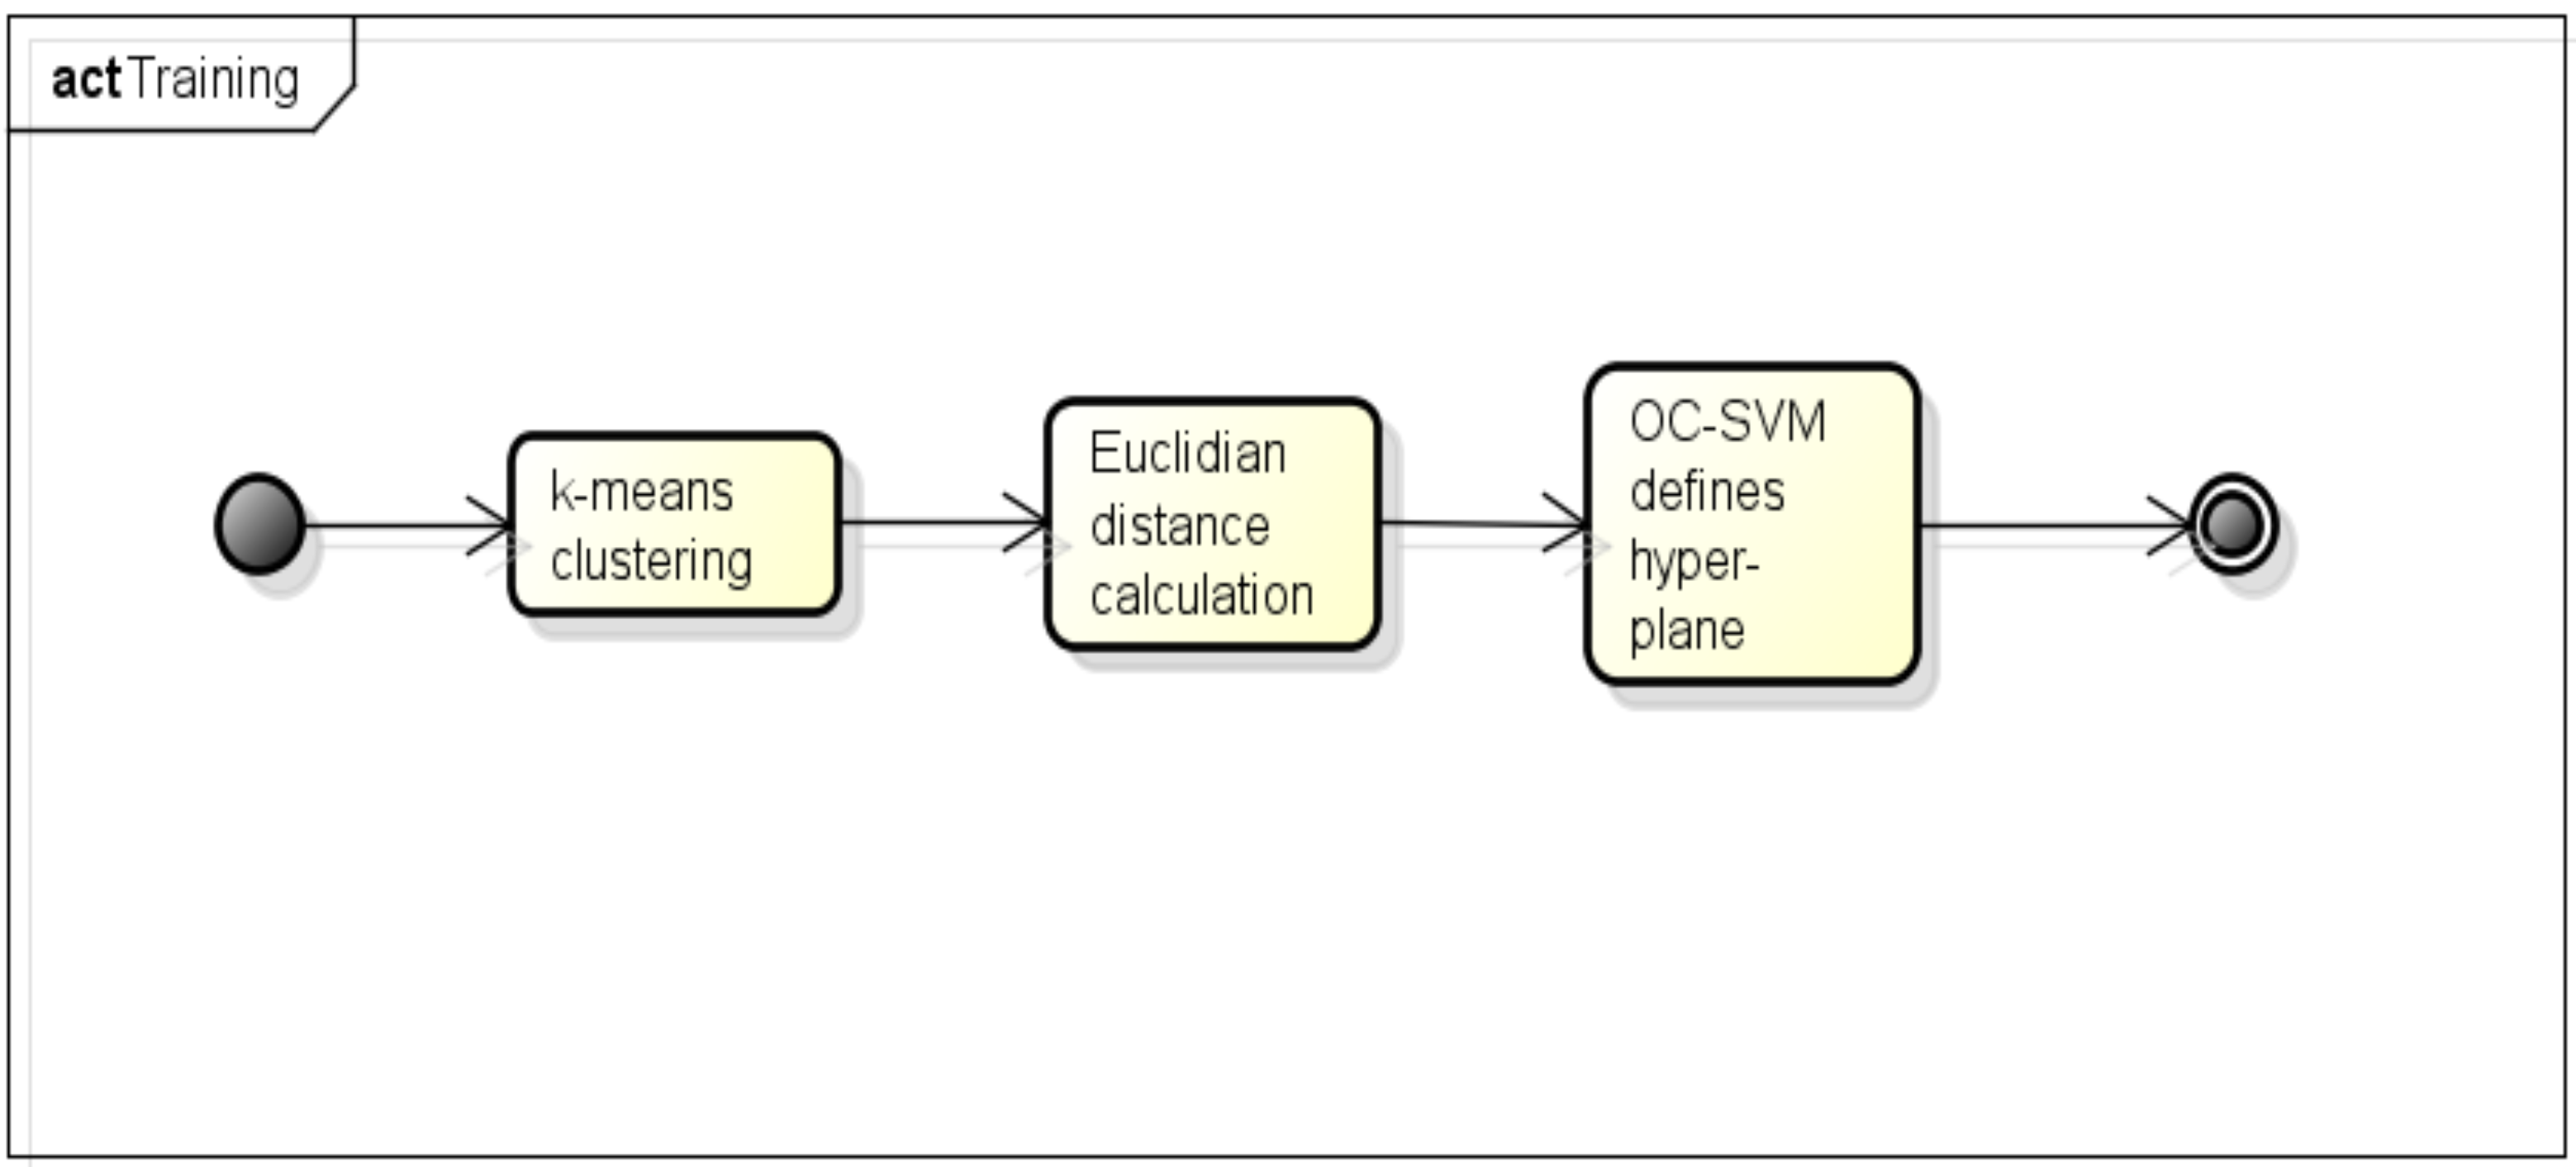
\includegraphics[scale=0.2068]{figures/ActivityDiagramTraining.png}
		  \caption{Activity diagram describing the training process of training component}
		  \label{fig:activityDiagramTraining}
		\end{figure}
				
		Additionally, Manandhar decided on the trade-off between false-positives and false-negatives in the sense that in order to minimise false-negatives, a higher false-positives rate is expected with the design of this IDS system \cite{Manandhar:TowardsPracticalAnomalyBasedIDS}.\ Therefore, the training component is not only responsible for the training process but also for the validation process, whose activity diagram is described in Figure~\ref{fig:activityDiagramValidation}.

		\begin{figure}[hb]
	 	 \centering
		  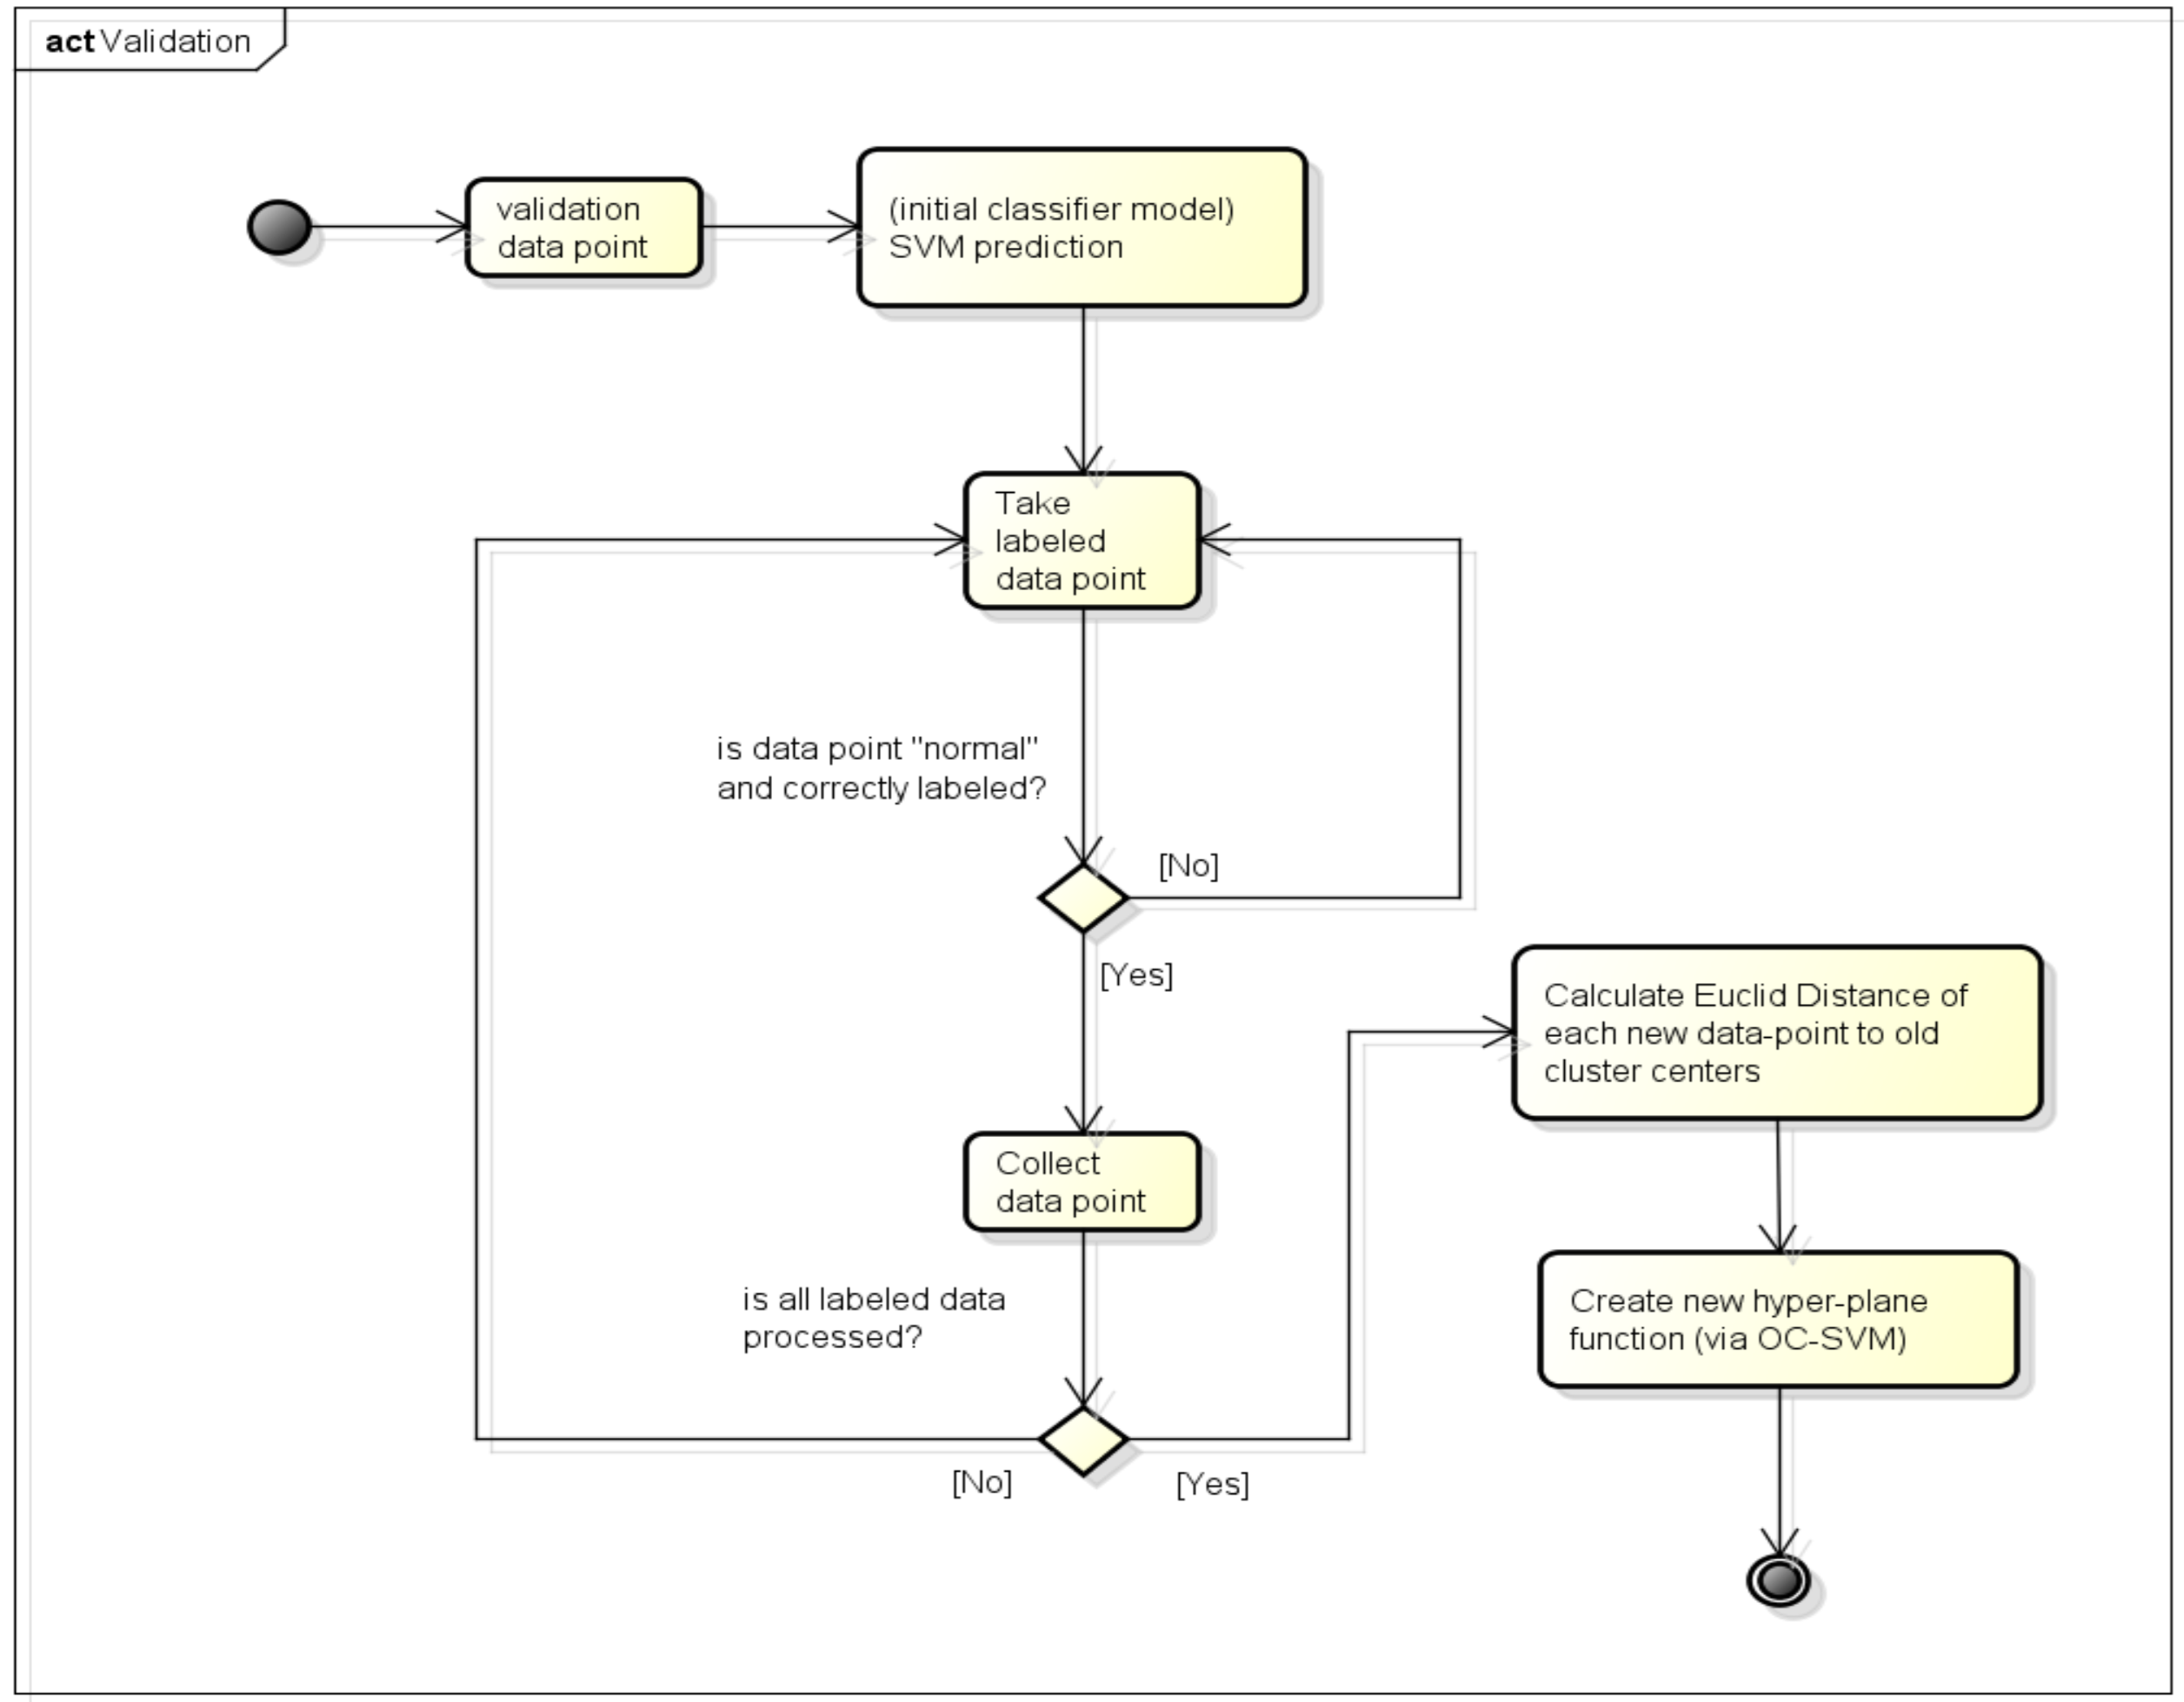
\includegraphics[scale=0.2668]{figures/ActivityDiagramValidation.png}
		  \caption{Activity diagram describing the validation process of training component}
		  \label{fig:activityDiagramValidation}
		\end{figure}
		
		The validation process aims to heightens the sensibility of the IDS detection capability.\ This is achieved by running the classification process on a validation data-set and only 'normal' data-points which were correctly classified by the IDS model (\textit{true positive}) is collected to construct the final IDS model whereas other data-points which were either anomaly or wrongly classified (\textit{true negatives}, \textit{false negatives}, and \textit{false positives}) are ignored and left out.
		
		Data-points collected during the validation process are analysed by calculating the distance of each data-point to all cluster centroids and the distance measure is used as an input for the one-class SVM to construct the final IDS model.

	\section{Classification Component}

		Based on the constructed final IDS model, the one-class SVM is able to classify new data-points.\ Beside the classification result, performance statistics is also collected in order to evaluate the IDS system afterwards.
		



\chapter{Implementation}
\label{implementation}

	Based on the approach of the authors explained in previous chapter, the implementation of the IDS system also consists of three parts, namely the implementation of data-set preprocessing component, training component, as well as classification component.\ The subsequent sections explain how each of these components are implemented and describe as well as explain any necessary changes which are made to the initial approach.

	\section{Data-Set Preprocessing Component}
	\label{dataSetPreprocessingComponent}
		
		The data-set preprocessing component is implemented to not only read the \textit{pcap\footnote{Pcap (packet capture) files are files that contains captured network traffic in form of network-packets.}} files from DARPA'$99$ data-sets but also to extract necessary relevant packet-headers from each network-packet in order to build feature vectors.\ Reading pcap files is assisted by the $Java$ library \textit{Pcap4J\footnote{Pcap4J is a $Java$ library that is able to work with different aspects of network-packet, including capturing, crafting and sending the network-packets.\ Homepage of Pcap4J: \url{http://www.pcap4j.org}}}, which is also able to extract the packet-header information.\ The extracted packet-header information is saved to the corresponding MySQL database, using the $Java$ standard SQL library.

		 As soon as all packet-header information is saved to the database, an aggregation of network-packets into TCP sessions is performed.\ This aggregation process is done by the means of SQL-aggregation query.\ Following the aggregation process is the dimension reduction of the feature vectors with the aids of PCA.\ However, due to lack of both know-how and experience as well as time limitation of this project, the authors decided to skip the dimension reduction process and proceeded with clustering process.\ Another reason to skip the PCA part is that the initial implementation of the dimension reduction process yields results that the authors are unable to understand and explain.\ Moreover, after several iterations of tests, the PCA part is determined to produce non-deterministic output which further encourages the authors to remove the dimension reduction process from the IDS system.\ By skipping the PCA part, the next step in the workflow is the training process which is handled by the training component.
		 
		 
	\section{Training Component}
	\label{trainingComponent}
		
		Building the initial as well as the final IDS model is the function of the training component.\ This component performs two main processes, namely the clustering process and the one-class SVM model building process, both of which are the core of the whole training as well as validation process.

		Clustering process is performed using k-means method with the help of \textit{Weka\footnote{Weka is a $Java$ library that contains a collection of machine learning algorithms such as PCA, K-means, as well as SVM.\ Homepage of Weka: \url{http://www.cs.waikato.ac.nz/~ml/weka/}}} library.\ Based on the work of Manandhar \cite{Manandhar:TowardsPracticalAnomalyBasedIDS}, the optimal cluster size for the DARPA'$99$ data-sets is three clusters, which is also the settings the authors agreed upon.\ Afterwards, the data-set preprocessing component calculate the Euclidian distance of each data-point in the training data-set to all three cluster centroids.\ As a result, each data-point contains three different distance measures, which are then utilised to build an initial IDS model.
		
		The one-class SVM takes the three distance measures of each data-point as input and constructs an IDS model which can be used as the classifier.\ Similar to k-means, the configuration of one-class SVM ($gamma$, $nu$, and $degree$) is also taken from the work of Manandhar \cite{Manandhar:TowardsPracticalAnomalyBasedIDS}.
		
		Based on the initial IDS model, the validation process is started by extracting building feature vectors from the validation data-set, followed by Euclidian-distance calculation of each validation data-point to the cluster centroids that are already built in the training process.\ Subsequently, the distance measures are used as input for the one-class SVM to classify the validation data-point.\ Every validation data-point that is classified as 'normal' and are actually normal (true negative), is collected and further utilised by the one-class SVM as the final IDS model.
		
	\section{Classification Component}
	\label{classificationComponent}
		 
		 As the name already suggests, the classification component is responsible for classifying a new data-point.\ This is done by utilising the final IDS Model supplied by the training component.\ Since the final IDS model contains only information about cluster distances, the IDS system has to trace back the data-point to the original aggregated TCP-session which contains valuable information necessary for the final output (alerts).\ Fortunately, the implemented IDS system works by preserving order of the data-points.\ Thus, the index of the final IDS model can be utilised to trace back to the original TCP-session contained in the database.\ Furthermore, the index makes it also possible to retrieve (available) labelling of the data-point so that performance statistics can be collected for the evaluation purposes.
\chapter{Results}
\label{results}

	Following the development process of the IDS system, an experiment was conducted in order to be able to objectively evaluate the performance of the IDS system.\ The evaluation process begins by choosing the (testing) data-set as input for the one-class SVM who is performing the classification based on the final IDS model.\ During the classification, several performance statistics such as \textit{true-positives\footnote{True-positives (TP) are data-points which are classified as anomalies and are actually anomalies.}}, \textit{true-negatives\footnote{True-negatives (TN) are data-points which are classified as normal and are actually normal.}}, \textit{false-positives\footnote{False-positives (FP) are data-points which are classified as anomalies but are actually normal.}}, \textit{false-negatives\footnote{False-negatives (FN) are data-points which are classified as normal but are actually anomalies.}}, as well as combinations of these measures, i.e. \textit{precision\footnote{$Precision = TP / (TP + FP)$}}, and \textit{recall\footnote{$Recall = TP / (TP + FN)$}}.\ This chapter explains the data-set that was chosen for the experiment and the evaluation result of the experiment.

	\section{Dataset Used}
	\label{datasetUsed}
	
		The publicly available DARPA'$99$ data-set is chosen for the experiment since this data-set is a widely popular benchmark for IDS and, thus, allows for comparison to other IDS-research works \cite{Manandhar:TowardsPracticalAnomalyBasedIDS}.\ As mentioned before in Chapter~\ref{background}, the DARPA'$99$ data-set consists of five weeks of data, where each week contains five days of collected network traffic.\ The conducted experiment works with three weeks of data, namely the first week, the fourth week and the fifth week as the training, validation and testing (classification) data-sets respectively.\ Since the first week data-set contains no attacks, it is most suitable to be used for the IDS training process, whereas the fourth as well as the fifth week data-sets contain attacks and are therefore used for validation and testing (classification) process.
		
		\subsubsection*{Labelling Attacks}
		\label{labellingAttacks}
			 In order for the developed IDS system to function properly, every attacks in the fourth and fifth week data-sets have to be labeled accordingly.\ The labelling of attacks in the data-sets serves the purpose of being able to evaluate the detection rate of IDS systems since otherwise the true-positives, true-negatives, false-positives, as well as false-negatives can not be determined.\ Unfortunately the search for such (machine-readable) labelling does not yield any promising results.\ This means that the validation process of the IDS system may produce non-ideal (potentially weak) final IDS model due to the fact that, without proper attacks labelling, the validation process might include false negatives (instead of only true-negatives) into the final IDS model.\ Additionally and most importantly, the evaluation process of the IDS system is also compromised.

		\subsubsection*{Partially Labelled Attacks}
		\label{partiallyLabelledAttacks}
		
			Nevertheless, the work of Manandhar \cite{Manandhar:TowardsPracticalAnomalyBasedIDS} also provides several SQL-scripts for attacks labelling.\ However, despite of identical database-structure, the SQL-scripts fails to label the attacks.\ Further analysis of the problem shows that the SQL-labelling-scripts contains time-offset.\ Consequently, the time-offset is readjusted\footnote{The time-offset readjustment is performed by adding $6$ hours of the \textit{packet-time} to each packet's time-stamp.} back to fit the original time-zone of the DARPA'$99$ data-sets.
			
			Even after the time-offset was readjusted, some of the SQL-labelling-scripts still can not label the attacks properly, for example the fourth week-labelling-script fails to label any attacks.\ Therefore, the SQL-labelling-scripts only work partially on the fifth week data-set.\ More precisely, only $63\%$ of $1000$ SQL-labelling-commands in the fifth week data-set is properly executed, which amounts to $159000$ successfully labelled attacks.

	\section{Evaluation}
	\label{evaluation}

		Testing the developed IDS system on the partially-labeled fifth week of DARPA'$99$ data-set yields a recall rate of $100\%$ and $30\%$ precision which is satisfying nevertheless since the high recall rate is the aim of the IDS system's architectural design \cite{Manandhar:TowardsPracticalAnomalyBasedIDS}.\ Moreover, with proper and complete attacks-labelling, a much higher precision rate can be achieved.
		
		It is also to be noted that the sensible IDS-system that achieves high detection rate always make the trade-off of having high false-positives as well, as in the developed IDS system within this project.\ In order to verify and/or estimate the false positive rate, the developed IDS system is given the first week of DARPA'$99$ data-set, which contains no attacks.\ As a result, $80\%$ of the data-points are labelled as normal, where as the rest were mis-labelled as anomalies, which corresponds to approximately $20\%$ false-positives.
\chapter{Conclusion}
\label{conclusion}

	During the course of this project all of the objectives set in chapter \ref{objectives} have been achieved and, therefore, the project goal was met.\ The authors have had first hand experience in the development of an IDS-system and how the focus-point of the IDS system can shape the architectural design which, in turn, may heavily determine the performance of the IDS system in regards of precision and recall rate.\ The missing attacks-labelling hinders the performance of the developed IDS system since the validation process requires labelled attacks in order to construct the final IDS model properly.
	
	Nevertheless the evaluation is performed on partly labelled data-set which results in succesfull identification of all attacks in the testing data-set.\ However, as described in Chapter~\ref{results}, such a high recall rate is accompanied with a low accuracy rate (high false-positives).\ Future works in this project might involve tinkering with the one-class SVM settings in order to achieve a higher accuracy rate with the minimal expense of lower recall rate.\ Additionally, introducing PCA into the IDS system properly may substantially decrease the required time to complete the training and validation process as currently the IDS system require approximately $10$ hours to perform the training and validation process.\ Lastly, a Graphical User Interface would increase the usability of the developed IDS system.
%\chapter*{Appendices}
\label{appendices}



%__________________________End_of_Thesis______________________________________________
\cleardoublepage
\addcontentsline{toc}{chapter}{Bibliography}
%harvard citations style, please uncomment harvard package in the usepackage area
%\bibliographystyle{agsm}
%remove the following line when using harvard style citation
\bibliographystyle{plain}
%specify bibtex file here
\bibliography{input/mybib}
%add appendix to TOC
%\addcontentsline{toc}{chapter}{Appendices}
%\input{input/07_appendix}

\end{document}
